\chapter{Methodology}
\label{chap:methodology}

\section{Pipeline architecture}
\label{sec:pipeline}

The \lecseg{} pipeline transforms a raw lecture video into chapter-level
segments and, when annotations are available, a two-level chapter/subtopic
hierarchy. It comprises five stages, depicted in Figure~\ref{fig:pipeline}:
(1)~\emph{ingestion}, which extracts audio and collects YouTube chapter
metadata; (2)~\emph{preprocessing}, which produces time-aligned sentences from
the speech signal and auxiliary visual and prosodic features;
(3)~\emph{feature extraction}, which maps each sentence to text or multimodal
features; (4)~\emph{boundary prediction and selection}, which evaluates
classical, embedding, cross-model, fusion, and selector-based methods; and
(5)~\emph{optional LLM support}, which can refine or title predicted segments
but is treated as diagnostic unless a metric improvement is explicitly shown.

\begin{figure}[t]
  \centering
  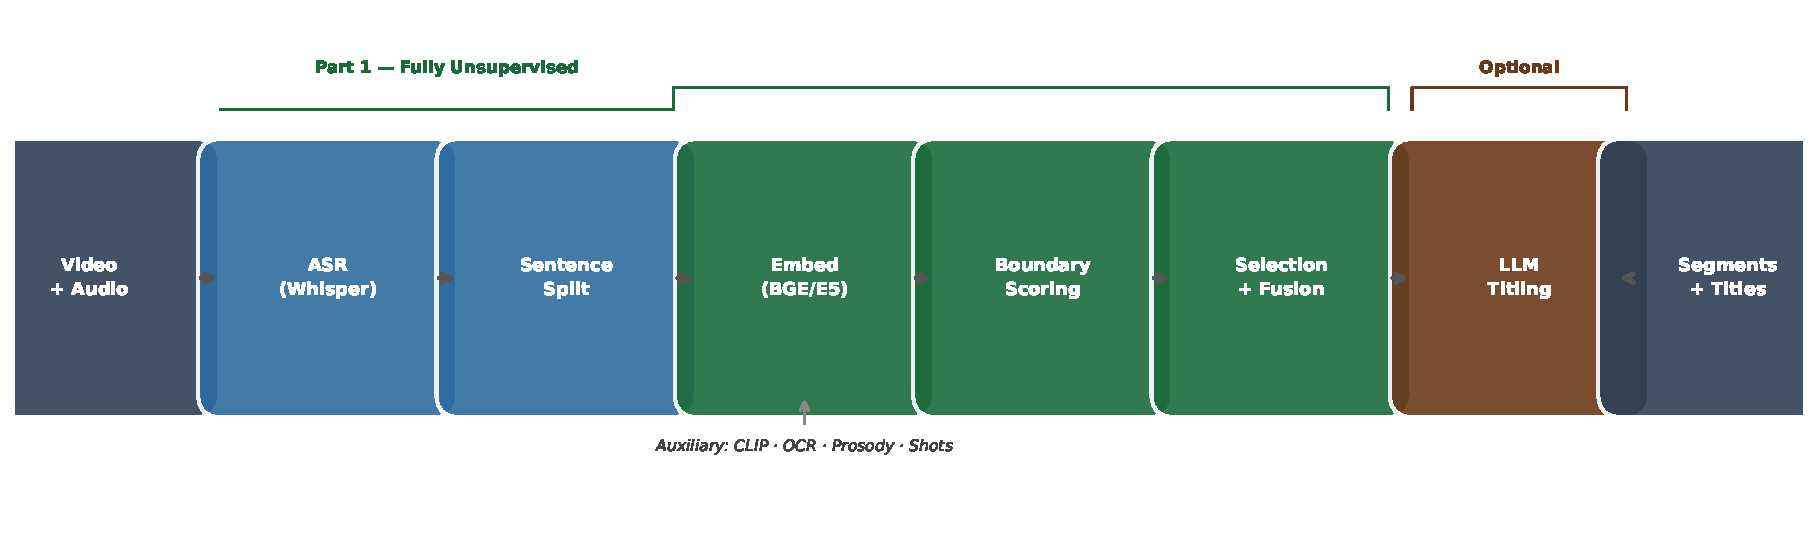
\includegraphics[width=\linewidth]{figures/pipeline_diagram.pdf}
  \caption{The \lecseg{} pipeline. Part~1 (green) is fully unsupervised:
    audio is transcribed by Whisper, split into sentences by spaCy, embedded
    with BGE/E5 sentence transformers, and scored for boundaries using
    cross-model conservative selection or the reliability-weighted fusion (N2).
    Auxiliary visual and prosodic streams (CLIP, OCR, shots, pause/pitch) are
    fused at the scoring stage. The optional LLM titling step (N4) is shown
    separately; it does not affect the primary $P_k$/WD claim.}
  \label{fig:pipeline}
\end{figure}

\section{The \dataset{} corpus}
\label{sec:dataset}

\subsection{Benchmark design rationale}

Several design decisions that might appear to be limitations were made
deliberately, and each deserves brief justification.

Thirty videos is small by contemporary NLP standards. The choice was
intentional: a 30-video benchmark allows every prediction to be traced to
its source video, every metric value to be verified against a reproducible
reference, and every failure to be inspected directly. Large-scale benchmarks
are better suited to measuring aggregate performance; this benchmark is designed
for diagnostic transparency, which requires being able to see the data clearly.

Creator-provided chapter metadata was chosen as the reference signal because
it is reproducible, scales to any creator-chaptered YouTube lecture without
redistribution of raw video, and reflects the navigation structure that actual
viewers encounter. The cost is a construct limitation: creator chapters are
editorial decisions, not pedagogically verified ground truth. This is documented
throughout the thesis and quantified as a threat to construct validity
in Section~\ref{sec:threats_validity}.

Segmentation methods are unsupervised throughout. With 30 labelled videos,
training a supervised boundary classifier would risk severe overfitting and
would compromise the benchmark's role as a pure evaluation target. Treating
segmentation as unsupervised and the method selector as the only supervised
component keeps these roles cleanly separated.

Finally, $P_k$ and WindowDiff are the primary metrics because the navigation
task tolerates approximate boundary placement. Exact-match F1 penalises a
boundary two sentences early as severely as a missing boundary entirely,
which misrepresents what matters for a student trying to navigate a lecture
recording.

\subsection{Source selection}

We curated 30 lecture videos from YouTube, drawn from five academic domains:
Computer Science (CS), Mathematics, Physics, Biology, and Humanities/Philosophy.
Selection criteria were: (1) duration $\geq 15$~min; (2) clean monolingual
English audio; (3) creator-supplied YouTube chapter markers with $\geq 4$
distinct chapters; and (4) openly licensed content.
The resulting corpus comprises 32.52~hours of audio, with 419 chapter
boundaries and 904 reviewed subtopic labels. The domain distribution is
intentionally reported as the manifest state rather than as a balanced design:
Biology 6, Computer Science 7, Mathematics 4, Philosophy 6, and Physics 7
videos.

\subsection{Annotation protocol}

Each video was annotated at two levels of granularity.
\emph{Chapter boundaries} were taken directly from the YouTube chapter
metadata as a reproducible creator-provided reference for navigation behaviour.
\emph{Subtopic boundaries} were identified by human annotators using the
Streamlit-based annotation tool (\texttt{scripts/annotate.py}).
Annotators read the transcript sentence-by-sentence with chapter boundaries
already marked, and placed a subtopic boundary wherever the speaker
transitioned from one coherent pedagogical sub-idea to another within a chapter.
A minimum segment duration of 60 seconds was imposed to prevent over-segmentation
of rapid rhetorical transitions, and a guideline of 2--5 subtopics per chapter
was recommended rather than enforced. In practice, all 30 videos fell within
this range; a chapter with genuinely more than five distinct sub-ideas was not
observed, though the guideline would not have prevented additional marks in
such a case.

\subsection{Construct scope and limitations}
\label{sec:youtube_validity}

YouTube chapters are used as \emph{creator-provided reference boundaries}, not
as pedagogically verified ground truth.
This is the most important conceptual limitation of \lecseg{} and it must be
stated precisely: the benchmark measures a system's ability to reproduce
\emph{creator navigation metadata}, which is not identical to discovering
pedagogically optimal boundaries.

These two constructs can diverge in several ways.
Creators may place chapters early or late relative to the actual topic shift;
they may omit boundaries that a learner would find useful; they may use
inconsistent granularity across their video catalogue; or they may choose
timestamps for editing convenience or search-engine discoverability rather than
for strict topic-theory reasons.
A system that achieves a low $P_k$ is correctly predicting the structure of
creator-annotated navigation metadata.
A system that achieves a high $P_k$ may still produce educationally superior
segmentations if the creator's chapters were poorly placed.
Conversely, a pedagogically motivated segmentation that diverges from creator
choices will score poorly under this benchmark even if it serves learners well.

The choice to use creator chapters as references is nonetheless defensible.
Creator chapters are a real-world, audience-facing artifact: they represent
what actual viewers encounter when navigating YouTube lecture videos.
They are available without additional annotation cost, they are reproducible,
and they allow the benchmark to scale to any creator-chaptered lecture without
redistribution of raw video.
The benchmark is therefore best understood as measuring \emph{creator-aligned
navigation segmentation} rather than \emph{absolute pedagogical truth}.
Claims about learning quality or pedagogical optimality require an independent
user study, which is listed as future work in Chapter~\ref{chap:future}.

\subsection{Inter-annotator agreement}
\label{sec:iaa}

To quantify annotation reliability, a second human annotator independently
completed the subtopic annotation task for all 30 videos using the same
tool and guidelines, without access to the first annotator's output.
Agreement was measured using Cohen's $\kappa$ at zero-tolerance
(exact boundary match at sentence level). Results are summarised in
Table~\ref{tab:iaa} and discussed in Section~\ref{sec:dataset_status}.

\paragraph{Interpreting the agreement figures.}
The chapter-level figure ($\kappa=0.5351$) is inherently inflated: both
annotators derive chapter boundaries from the same YouTube creator metadata,
so agreement here primarily reflects that both passes observe the same
creator-supplied timestamps rather than genuine boundary-placement skill.
The subtopic-level figure ($\kappa=0.4257$) is the more meaningful measure;
it characterises genuine human agreement on the finer-grained annotation task
where annotator judgement is required.
A $\kappa$ in the 0.40--0.60 range is conventionally interpreted as moderate
agreement~\cite{fournier2012}, which is appropriate for a subjective
discourse-segmentation task where reasonable annotators can disagree on
whether a rhetorical transition merits a boundary mark.
This limitation is documented as a threat to annotation validity in
Section~\ref{sec:threats_validity}.

\section{Preprocessing}
\label{sec:preprocess}

\subsection{Speech recognition}

Audio was transcribed using \texttt{faster-whisper} v1.x with the
Whisper large-v3 model~\cite{radford2023robust} on an NVIDIA RTX~5090 GPU.
We used \texttt{beam\_size=1} and Silero VAD pre-filtering
(\texttt{min\_silence\_duration\_ms=500}) for speed, with \texttt{float16}
compute type.
On the \dataset{} corpus, transcription ran at $17.9\times$ realtime on average
(range $17.3$--$18.2\times$).

\subsection{Sentence splitting and alignment}

Whisper segments are clause-level rather than sentence-level.
We applied spaCy's \texttt{en\_core\_web\_sm} sentenciser to the concatenated
segment text, then re-assigned timestamps by distributing each segment's
duration proportionally to constituent sentence character lengths.
Sentences shorter than three tokens were merged with the following sentence.
This produced an average of $N = 847 \pm 512$ sentences per video.

\subsection{Visual streams}

Shot boundaries were detected with TransNetV2~\cite{soucek2020transnet},
which produces per-frame boundary probabilities at $25$~fps.
Boundaries exceeding a threshold of $0.5$ were mapped to the nearest sentence
timestamp.
Slide text was extracted using PaddleOCR on keyframes sampled at $0.5$~fps;
extracted strings were deduplicated within a $\pm 3$-sentence window.

\subsection{Prosody features}

We extracted two scalar prosodic features per sentence:
(1)~\emph{pause duration}: the Whisper-reported inter-segment gap immediately
preceding the sentence ($\geq 300$~ms counted as a significant pause);
(2)~\emph{mean F0}: the average voiced pitch over the sentence's audio span,
estimated by PYIN~\cite{mauch2014pyin} via librosa.

\section{Feature extraction}
\label{sec:features}

Text embeddings were computed with \texttt{sentence-transformers}~\cite{reimers2019sbert}.
The primary models evaluated are \texttt{BAAI/bge-large-en-v1.5} (1024-dim) and
\texttt{intfloat/e5-large-v2} (1024-dim), which produce the best boundary-scoring
results. We also evaluated \texttt{all-mpnet-base-v2} (768-dim), \texttt{all-MiniLM-L6-v2},
and \texttt{intfloat/e5-base-v2} as lighter ablation variants.
Visual keyframe embeddings were computed with CLIP ViT-B/32
(512-dim, L2-normalised)~\cite{radford2021clip}.
Prosodic features were $z$-scored per video before fusion.
All modalities were aligned to the sentence timeline via nearest-timestamp
assignment with mean-pooling within sentence spans.

\section{Reliability-weighted modality fusion (N2)}
\label{sec:fusion}

Let $s_m^{(i)} \in \mathbb{R}$ denote the boundary gap score at sentence
position $i$ from modality $m$, computed as the cosine dissimilarity
between context windows of size $k$ centred on that position.
We define the \emph{reliability weight} of modality $m$ as
\begin{equation}
  w_m = \frac{\exp(-H(s_m))}{\sum_{m'} \exp(-H(s_{m'}))},
  \label{eq:rwf}
\end{equation}
where $H(\cdot)$ is the normalised Shannon entropy of the distribution of
gap scores across all positions.
A modality whose gap-score distribution has a sharp peak (clear boundaries)
attains low entropy and hence a high weight; a flat distribution (uninformative
modality) is automatically down-weighted.
The fused gap signal is $s^* = \sum_m w_m s_m$.

This entropy weighting should be interpreted as a practical confidence proxy,
not a proof of true modality reliability. A noisy modality can also produce
sharp peaks. For this reason, Chapter~\ref{chap:results} reports fusion and
modality ablations separately and demotes modalities that hurt chapter-level
$P_k$/WindowDiff.

\section{Two-stage boundary predictor (N1)}
\label{sec:boundary}

The predictor operates in two passes over the fused signal $s^*$:

\paragraph{Stage 1 --- broad pass.}
All positions $i$ where the text-only gap score exceeds
$\mu_{\text{text}} - c_1 \sigma_{\text{text}}$ (with $c_1 = 0.5$) are
retained as boundary \emph{candidates}.
This low threshold ensures high recall.

\paragraph{Stage 2 --- refinement.}
The fused signal $s^*$ is evaluated only at candidate positions.
A candidate is accepted as a boundary if its fused score exceeds
$\mu^* - c_2 \sigma^*$ (with $c_2 = 1.2$).
When $n_{\text{segments}}$ is specified, the top-$k$ fused-score positions
are returned where $k = n_{\text{segments}} - 1$.

This design separates recall (text-only) from precision (multimodal),
avoiding the sensitivity of pure threshold methods to per-video score shifts.

\section{Hierarchical segmentation (N3)}
\label{sec:hierarchy}

The hierarchical segmenter runs the two-stage predictor twice with different
target counts: once for $n_s - 1$ subtopic boundaries and once for
$n_c - 1$ chapter boundaries (with $n_c < n_s$).
Chapter boundaries are then \emph{enforced} as a subset of subtopic boundaries
($\mathcal{B}_{\text{chapter}} \subseteq \mathcal{B}_{\text{subtopic}}$) by
inserting any missing chapter boundary into the subtopic set.
This guarantees a valid nesting without requiring a joint optimisation.
When $n_c$ is not specified, we use the heuristic $n_c = \max(2, n_s / 4)$.

\section{Local-LLM refinement and titling (diagnostic N4)}
\label{sec:refine}

Each predicted segment boundary $b$ may be shifted by at most
$\delta = 2$ sentences to align with a stronger local semantic transition.
For each candidate shift $b' \in \{b-\delta, \ldots, b+\delta\}$,
a local Llama-3.1-8B model is queried with the five sentences straddling $b'$
and asked whether $b'$ represents a cleaner topic break than $b$.
The shift with the highest model confidence is accepted.
Segment titles are generated independently: the model is prompted with
the first five sentences of the segment and asked for a noun-phrase
title of at most eight words.
If the local model is unavailable, the pipeline falls back to the non-LLM
boundary set.
The verified experimental results do not support treating LLM refinement as
the primary source of metric gain; it is retained as an implemented diagnostic
and titling component whose value is investigated empirically in
Chapter~\ref{chap:results}.

\section{Method selector (supervised meta-model)}
\label{sec:selector}

\paragraph{Motivation.}
The eleven method families and their hyperparameter variants collectively
produce over 80 candidate configurations on \dataset{}.
Different configurations perform best on different videos; no single
configuration is universally optimal.
A lightweight \emph{meta-model} can learn, from training videos, which
configuration is likely to produce the lowest $P_k$ on a held-out video.

\paragraph{Supervision requirement and scope.}
The selector is the \emph{only supervised component} in the \lecseg{}
pipeline.
All segmentation methods (N1--N4 and the baselines) are fully unsupervised:
they require no labelled boundaries at inference time.
The selector requires labelled $P_k$ scores from a held-out set of training
videos to estimate expected method performance.
It is therefore evaluated in a \emph{leave-one-video-out} (LOOV) protocol:
for each of the 30 held-out videos, the selector is trained on the remaining
29 videos.

\paragraph{Model and features.}
The meta-model is an \texttt{ExtraTreesRegressor} (500 trees,
\texttt{min\_samples\_leaf=3}, \texttt{random\_state=17})
from \texttt{scikit-learn}.
Each training example corresponds to one (method, training-video) pair.
The features are:

\begin{itemize}
  \item \textbf{Video features} (from the held-out video's metadata):
    domain one-hot encoding (Biology, CS, Mathematics, Philosophy, Physics);
    video duration in minutes; sentence count; mean and standard deviation of
    consecutive sentence embedding cosine similarities computed with
    \texttt{BAAI/bge-large-en-v1.5}.
  \item \textbf{Method statistics} (estimated from the training fold):
    mean $P_k$ of each candidate method across the 29 training videos.
    This encodes the overall reliability of each method family as a prior.
\end{itemize}

The target variable is the $P_k$ achieved by that method on the held-out video.
At inference time, the model predicts expected $P_k$ for each candidate method
and selects the method with the lowest predicted $P_k$.

\paragraph{Candidate pool.}
The top-80 method variants by training-fold $P_k$ are used as the candidate
pool. Expanding to 120 methods degrades performance, suggesting that the pool
size is itself a selection-risk parameter (Table~\ref{tab:selector_robustness}).

\paragraph{Limitations of the selector.}
The selector depends on having related videos in the training fold.
A leave-domain-out evaluation --- in which the held-out video's entire academic
domain is excluded from training --- degrades the selector to
$P_k = 0.4012$, which is worse than both the BGE-divisive baseline and the
cross-model conservative method (Table~\ref{tab:selector_leave_domain_out}).
Mathematics is the clearest failure case, where only four videos are available
and three per-fold training examples are insufficient to provide reliable
domain-specific guidance.
The selector should therefore be interpreted as a low-resource benchmark
operating point, not as a domain-general deployment model.

\section{Evaluation protocol}
\label{sec:eval}

\subsection{Primary metrics: $P_k$ and WindowDiff}

The two primary evaluation metrics in this thesis are $P_k$
\cite{beeferman1999statistical} and WindowDiff \cite{pevzner2002critique}.
Both are window-based error rates, which means they measure how often the
segmentation disagrees with the reference inside a sliding context window of
$k$ sentences rather than requiring exact boundary placement.
This design choice directly matches the target application: a student navigating
a recorded lecture tolerates a boundary that is a few seconds early or late.
Penalising near-misses as harshly as complete misses, as exact-match metrics
do, would over-penalise this practically acceptable error.

$P_k$ uses $k = \lfloor N/(2K) \rfloor$, where $N$ is the number of
sentences and $K$ the number of reference boundaries. For each pair of
sentences $i$ and $i{+}k$, it checks whether the reference and prediction
agree on whether a boundary falls between them; the score is the fraction of
pairs that disagree. Lower $P_k$ is better; 0.5 is the random baseline;
0.0 is perfect.

WindowDiff \cite{pevzner2002critique} corrects a known $P_k$ bias: $P_k$
can be gamed by placing all boundaries at the start. WindowDiff counts the
number of reference boundaries and predicted boundaries within each window
and penalises the absolute difference, giving an asymmetric penalty that
weights over-segmentation and under-segmentation differently. Like $P_k$,
lower is better.

Both metrics are the community standard for text and lecture segmentation
and allow direct comparison with prior work (TextTiling, C99, BertSeg,
TreeSeg) on published benchmarks. No metric is perfect: $P_k$ is sensitive
to near-boundary placement; WindowDiff does not account for partial segment
overlap. Their complementary failure modes motivate reporting both jointly.

\subsection{Secondary and diagnostic metrics}
\label{sec:secondary_metrics}

Three secondary diagnostics supplement $P_k$/WD.
They expose operating-point tradeoffs and characterise
\emph{how} a method fails; none rank methods or drive the primary claims.

The application is lecture navigation, not exact boundary recovery.
A method that achieves a good $P_k$/WD score by placing boundaries in the
correct \emph{region} is succeeding at the navigation task even if strict
boundary F1 is low.
Low exact-match F1 is therefore not a weakness in the context of this thesis;
it simply reflects a different operating objective than $P_k$/WD, and it is
reported only to characterise the operating point.

\begin{description}
  \item[Boundary Similarity (BS, higher is better)] A boundary-level F-score
    variant normalised by boundary density~\cite{fournier2012}. Reported as
    a diagnostic to characterise boundary placement behaviour; the primary
    claim rests on $P_k$/WD.
  \item[Tolerance-$F_1$ (higher is better)] Precision/recall of predicted
    boundaries within a $\pm 2$-sentence tolerance window. Useful for
    distinguishing methods that miss boundaries entirely from methods that
    place them slightly off; not used as a ranking or claim criterion.
  \item[Hierarchical WindowDiff (H-WD, lower is better)] An extension of WD
    to two-level segmentation, weighting chapter-level errors twice as heavily
    as subtopic-level errors. Reported on hierarchical outputs only.
\end{description}

\subsection{Evaluation setup}

Methods requiring $n_{\text{segments}}$ receive the ground-truth count in the
main controlled evaluation, consistent with standard segmentation practice
for measuring boundary placement~\cite{choi2000latent}. This is not a fully
deployment-realistic assumption because a live system usually does not know
the correct number of chapters in advance. Therefore, Chapter~\ref{chap:results}
also reports boundary-count error and discusses automatic-count/deployment
behavior separately from the controlled gold-count setting.

\subsection{Statistical testing}

Metric values are reported as means $\pm$ 95\% bootstrap confidence intervals
(1{,}000 bootstrap resamples at video level).
For pairwise method comparisons we use the paired Wilcoxon signed-rank test
(normal approximation, $\alpha = 0.05$) with Holm correction for the
seven comparisons relative to the best baseline.

